% ============================================================
% main.tex — IEEE Access submission
% LLM-Augmented Azure VM Incident Triage with RAG Memory
% and Online Self-Learning
% ============================================================
\documentclass[a4paper,10pt,journal,compsoc]{IEEEtran}

% --- Encoding & fonts ---
\usepackage[T1]{fontenc}
\usepackage[utf8]{inputenc}

% --- Core IEEE packages ---
\usepackage{cite}
\usepackage{amsmath,amssymb,amsfonts}
\usepackage{algorithmic}
\usepackage{graphicx}
\usepackage{textcomp}
\usepackage{xcolor}

% --- Tables ---
\usepackage{booktabs}
\usepackage{multirow}

% --- Links ---
\usepackage{hyperref}
\usepackage{url}

% --- TikZ / PGF ---
\usepackage{tikz}
\usepackage{pgfplots}
\pgfplotsset{compat=1.18}
\usetikzlibrary{shapes.geometric, arrows.meta, positioning,
  fit, backgrounds, decorations.pathreplacing,
  calc, matrix, shadows}

% --- Code listings ---
\usepackage{listings}
\lstset{
  basicstyle=\ttfamily\footnotesize,
  frame=single,
  breaklines=true,
  keywordstyle=\color{blue},
  stringstyle=\color{orange},
  commentstyle=\color{gray},
  showstringspaces=false
}

% --- BibTeX logo ---
\def\BibTeX{{\rm B\kern-.05em{\sc i\kern-.025em b}\kern-.08em
    T\kern-.1667em\lower.7ex\hbox{E}\kern-.125emX}}

% ============================================================
\begin{document}

\title{LLM-Augmented Azure VM Incident Triage with RAG Memory\\
and Deterministic Safety Enforcement}

\author{%
  \IEEEauthorblockN{Mohammed Ilham}
  \IEEEauthorblockA{\textit{Dept.\ of Computer Science and Engineering}\\
    \textit{R.V.\ College of Engineering}\\
    Bengaluru, India\\
    mohammedilham.cs22@rvce.edu.in}
  \and
  \IEEEauthorblockN{Smriti Srivastava}
  \IEEEauthorblockA{\textit{Dept.\ of Computer Science and Engineering}\\
    \textit{R.V.\ College of Engineering}\\
    Bengaluru, India\\
    smritis@rvce.edu.in}
}

\maketitle

% ============================================================
% ABSTRACT
% ============================================================
\begin{abstract}
Cloud infrastructure incidents at scale demand triage systems that are
both fast and accurate. Rule-based AIOps systems handle known failure
patterns reliably but often fail to classify incidents outside their
encoded rule coverage, while large
language models (LLMs) introduce hallucination risk that can produce
dangerous remediation suggestions. This paper presents a six-layer
read-only architecture for Azure VM incident triage that combines a
deterministic rule engine, dual-collection retrieval-augmented
generation (RAG) memory, structured LLM reasoning with provider
fallback, and a deterministic post-LLM safety guard enforcing six hard
safety rules. We evaluate the system on a 100-case synthetic benchmark
spanning 23 known incident patterns and 5 novel patterns, constructed
from Azure documentation and public SRE runbooks. The rule engine with
safety guard achieves 88.0\% accuracy (88/100), while removing the
safety guard reduces accuracy to 82.0\%, primarily because
platform-event cases are no longer correctly forced to abstention.
LLM-only triage achieves lower overall accuracy (73.0\%) but higher
novel-pattern accuracy than the rule baseline (60.0\% vs 20.0\%),
indicating potential value for unseen incidents. LLM+SOP RAG and the
full system each achieve 86.0\% accuracy in the static benchmark,
suggesting that incident memory provides limited benefit in one-pass
evaluation. In a separate 20-case longitudinal experiment,
novel-pattern accuracy improves from 20.0\% to 80.0\% over five
feedback-driven memory-update cycles, though the small novel subset
($n=5$) makes this result directional rather than conclusive. The
safety guard intercepts all~30 hand-crafted unsafe suggestions in the
adversarial test set and produces no false blocks on healthy benchmark
VMs. These results suggest that deterministic post-generation safety
checks and feedback-driven retrieval memory are feasible design
patterns for LLM-assisted cloud triage, but real incident validation
and independent expert labeling remain necessary.
\end{abstract}

\begin{IEEEkeywords}
AIOps, incident management, incident triage, large language models,
retrieval-augmented generation, LLM safety, decision support,
cloud operations, Azure
\end{IEEEkeywords}

% ============================================================
\section{Introduction}
% ============================================================

\subsection{Problem Statement}

Cloud infrastructure downtime carries severe financial and operational
consequences. Industry surveys place the average cost of high-impact
unplanned data-centre outages in the hundreds of thousands of dollars
per hour, with the most disruptive events reaching seven-figure
totals~\cite{uptime2023outage}. Hyperscale
cloud providers manage millions of virtual machine instances across
global regions. At this scale, even a 0.1\% incident rate generates
thousands of simultaneous alerts, far exceeding the capacity of on-call
engineering teams to triage manually. Automated incident triage is
therefore not a convenience but an operational necessity.

Current AIOps systems for cloud VM triage are predominantly rule-based.
Azure Monitor alert rules, Prometheus AlertManager, and similar
platforms apply deterministic threshold conditions to telemetry
streams: if CPU exceeds 95\% for five minutes, fire an alert. These
systems are fast, auditable, and reliable for known failure patterns.
However, they require manual threshold tuning for each metric, cannot
generalize across correlated multi-signal failures, and often produce
no useful output when incidents involve patterns not anticipated at
rule-authoring time.
In practice, novel failure modes---new OS versions, unexpected
interaction effects between services, infrastructure changes---account
for a disproportionate share of high-severity incidents precisely
because they are not covered by existing rules~\cite{chen2024rcacopilot}.

Large language models offer a compelling alternative for novel pattern
reasoning. An LLM can read free-form telemetry, reason over signal
combinations, and generate contextually appropriate remediation
suggestions without requiring explicit rule definitions. However, LLMs
introduce a critical risk in production operations: hallucination. An
LLM that confidently suggests restarting a VM during an active platform
maintenance window, or recommends deleting an OS disk based on
ambiguous signals, can cause data corruption or extended downtime that
is worse than the original incident. Few published systems describe
deterministic post-generation safety enforcement for LLM-generated
cloud remediation suggestions in sufficient detail to evaluate its
effect on triage safety.

The gap this paper addresses is the absence of a system that combines:
(a)~a strong deterministic rule baseline for known patterns,
(b)~LLM reasoning for novel patterns,
(c)~RAG memory for cumulative knowledge accumulation without
retraining, and
(d)~deterministic post-LLM safety enforcement that cannot be bypassed
by any LLM output. We present such a system and evaluate it empirically
on 100 benchmark cases.

\subsection{Contributions}

\begin{enumerate}
\item A 6-layer architecture for LLM-assisted Azure VM incident triage
  that combines a deterministic rule baseline, dual-collection RAG
  memory, structured LLM reasoning, and a deterministic post-LLM safety
  guard. On a 100-case synthetic benchmark the rule engine with safety
  guard reaches 88.0\% overall accuracy; a safety-guard ablation shows
  a 6-percentage-point improvement (82.0\%~$\to$~88.0\%).
\item A dual-collection RAG design that separates static SOP knowledge
  from a growing incident memory of human-verified resolutions, enabling
  \emph{feedback-driven memory updates} without any LLM retraining. In
  a longitudinal evaluation on a 20-case held-out set, novel-pattern
  accuracy rises from 20.0\% to 80.0\% over five cycles of memory
  growth; we deliberately avoid calling this ``learning'' because no
  model weights change.
\item A deterministic, post-LLM safety guard that applies six hard
  safety rules as an unconditional override. Against 30 hand-crafted
  adversarial suggestions spanning all six rules the guard intercepts
  every one; on the 100-case benchmark it produces no false blocks on
  healthy VMs. We position this as an \emph{important} architectural
  component under the evaluated conditions, rather than a necessary one
  in the absolute sense.
\item A reproducibility-oriented synthetic benchmark of 100 cases spanning 23
  known patterns and 5 novel patterns, together with evaluation scripts,
  per-case detail records, and safety-ablation results, so that the
  claims in Section~4 can be independently re-verified.
\end{enumerate}

% ============================================================
\section{Related Work}
% ============================================================

\subsection{Rule-Based AIOps}

Threshold-based alerting has been the backbone of IT operations
monitoring for over two decades. Systems such as Nagios, Prometheus
AlertManager, and Azure Monitor native alert rules evaluate
deterministic conditions against telemetry streams and fire alerts when
thresholds are breached. Critically, their primary advantages---speed,
auditability, and zero false-negative rate for known patterns---come
with a structural cost: every failure mode must be anticipated and
encoded at rule-authoring time. Azure Monitor, for example, supports
metric alert rules, log-based alerts, and activity log alerts, all
evaluated deterministically against pre-configured
thresholds~\cite{microsoft2024azuremonitor}. A broader survey of AIOps
failure-management techniques~\cite{notaro2021aiops} distinguishes
detection, localisation, and remediation stages, and observes that most
production deployments remain detection- and correlation-oriented, with
remediation still largely operator-driven. Log-based anomaly
detection approaches~\cite{shi2021log} and multivariate time-series
anomaly detection on service-level metrics~\cite{ma2021jumpstarting}
further illustrate the state of practice before LLM-based reasoning
was introduced.

Microsoft's internal AIOps research has explored automated alert
correlation, noise reduction, and root cause analysis at
scale~\cite{ahmed2023rootcause,xu2024xlifecycle}. These systems apply
machine learning to cluster related alerts and reduce alert fatigue,
but they remain fundamentally reactive: they classify and correlate
known alert types rather than reasoning about novel failure patterns.
The RCACopilot system~\cite{chen2024rcacopilot}
demonstrates automated on-call incident diagnosis using LLM-based root
cause analysis at Microsoft, but focuses on software service incidents
rather than infrastructure-level VM triage and does not address safety
enforcement.

The fundamental limitation of rule-based AIOps is brittleness: rules
must be manually authored for each failure pattern, require ongoing
maintenance as infrastructure evolves, and produce no output for
incidents outside their coverage. The Google SRE
Book~\cite{beyer2016sre} acknowledges this limitation, noting that
novel failure modes are disproportionately represented in
high-severity incidents. Our system addresses this gap by combining a
rule engine for known patterns with LLM reasoning for novel ones.

\subsection{LLM for Incident Management}

In contrast to rule-based approaches, large language models offer
generalization across unseen failure patterns. Built on transformer
architectures~\cite{vaswani2017attention,devlin2019bert}, modern LLMs
can read free-form telemetry, reason over signal combinations, and
generate contextually appropriate remediation suggestions without
requiring explicit rule definitions. Notably, chain-of-thought
prompting~\cite{wei2022cot} enables LLMs to decompose complex
diagnostic reasoning into intermediate steps---a property we exploit
in our structured prompt design (Section~\ref{sec:layer6}).

Domain-specific LLMs for IT operations have emerged as a distinct
research direction. OWL~\cite{guo2024owl} is a large language model
trained specifically on IT operations data, demonstrating that
domain-specific pre-training improves performance on operational tasks.
GPT-4~\cite{openai2023gpt4} and its successors have been applied to
automated root cause analysis~\cite{zhang2023automated}, with
promising results on cloud incident datasets. A comprehensive survey
of LLM applications in cloud incident management~\cite{zeng2023aiops}
identifies incident triage as a high-value use case but notes that
production deployment remains limited due to reliability and safety
concerns.

Commercial systems such as Microsoft Copilot for Azure and GitHub
Copilot for Operations provide LLM-assisted incident investigation,
but these systems operate in advisory mode---they suggest actions for
human review rather than making autonomous triage decisions. This
design choice reflects the core challenge: LLMs fail to reliably
self-correct errors in their own reasoning~\cite{huang2024selfcorrect},
a limitation that extends to safety-critical suggestion
generation---an LLM that produces an unsafe remediation step cannot be
relied upon to detect and retract it without an external guard.

\subsection{Retrieval-Augmented Generation in Operations}

Retrieval-Augmented Generation (RAG), introduced by Lewis et
al.~\cite{lewis2020rag}, augments LLM generation with retrieved
context from an external knowledge store. The underlying embedding
technology traces to dense vector representations of
text~\cite{mikolov2013word2vec}, refined through transformer-based
sentence encoders~\cite{devlin2019bert} and ultimately the
Sentence-BERT architecture~\cite{reimers2019sbert} that underpins the
\texttt{all-MiniLM-L6-v2} model we use. RAG addresses the knowledge
staleness problem inherent in static LLM training: by retrieving
relevant documents at inference time, the system can incorporate
information that postdates the model's training cutoff without
retraining.

In IT operations, RAG has been applied to runbook retrieval, SOP
grounding, and incident post-mortem analysis. Toro Isaza et
al.~\cite{isaza2024ragitsupport} demonstrate that RAG-augmented
incident resolution systems outperform pure LLM approaches on IT
support tasks by providing grounded, verifiable context from historical
tickets. Our system extends this approach with a dual-collection
architecture: one ChromaDB collection for SOP knowledge (static,
curated) and one for incident memory (dynamic, grows with each resolved
incident). Human-verified cases are prioritized in retrieval, ensuring
that confirmed resolutions rank above unverified LLM outputs.

A key advantage of RAG over fine-tuning for operational systems is
online updateability. Fine-tuning requires retraining cycles that may
take hours to days, while RAG memory updates are instantaneous---a
resolved incident is available for retrieval within seconds of being
stored. This property is what enables the feedback-driven memory-update
loop described in Section~\ref{sec:layer6}; we deliberately avoid the
term ``learning'' for this loop because no model weights are updated.

\subsection{Safety Enforcement in Agentic AI Systems}

As LLM-based agents gain the ability to take actions with real-world
consequences, safety enforcement has emerged as a critical research
area. Constitutional AI~\cite{bai2022constitutional} proposes training
LLMs with explicit safety principles, but this approach relies on the
model's learned behavior and cannot provide hard guarantees---red-teaming
studies~\cite{perez2022redteaming} and automated adversarial-suffix
attacks~\cite{zou2023universal} have shown that sufficiently adversarial
prompts can still elicit unsafe outputs from constitutionally trained
models.

For cloud infrastructure operations, the stakes of unsafe actions are
particularly high. Restarting a VM during a platform maintenance window
can cause data corruption. Deleting an OS disk based on ambiguous
signals is irreversible. Disabling NSG rules to ``debug connectivity''
exposes the VM to the public internet. These actions share a common
property: they are easy to suggest, difficult to reverse, and
potentially catastrophic.

Our approach complements learned safety with a deterministic, post-LLM
safety guard that applies six hard rules as a final override layer.
The guard is not a prompt instruction or a fine-tuned behavior---it is
imperative code that runs after LLM output is generated and cannot be
bypassed by any LLM output, including prompt-injection or suffix
attacks. This design provides hard enforcement for the specified rule
classes, at the cost of some flexibility in
edge cases where the safety rules may be overly conservative. We
position the guard as an important architectural component for the
settings we evaluate, rather than as a universally necessary one;
establishing necessity in a stricter sense would require head-to-head
comparison with prompt-only, constrained-decoding, and
classifier-validator alternatives, which we leave to future work.

% ============================================================
\section{System Architecture}
% ============================================================

\begin{figure*}[!t]
  \centering
  % fig4_architecture.tex
% 6-layer pipeline diagram for IEEE Access paper
% Include in main.tex with: % fig4_architecture.tex
% 6-layer pipeline diagram for IEEE Access paper
% Include in main.tex with: % fig4_architecture.tex
% 6-layer pipeline diagram for IEEE Access paper
% Include in main.tex with: \input{fig4_architecture}
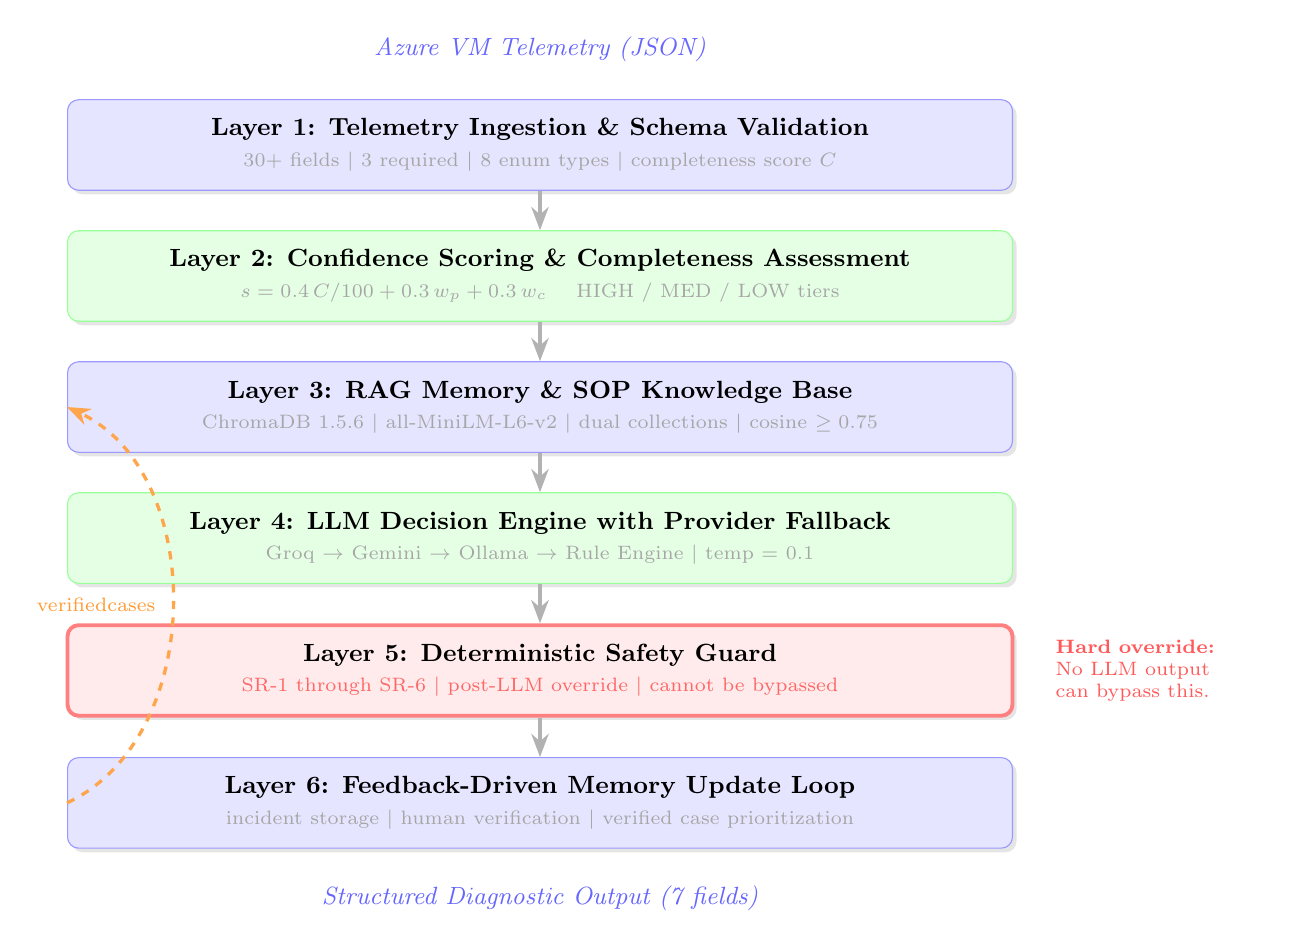
\begin{tikzpicture}[
  node distance=0.5cm,
  layer/.style={
    draw, rounded corners=4pt,
    minimum width=12cm, minimum height=1.15cm,
    align=center, font=\small\bfseries,
    drop shadow={shadow xshift=1.5pt, shadow yshift=-1.5pt,
                 fill=black!20, opacity=0.5}
  },
  arrow/.style={-Stealth, thick, gray!60, line width=1.2pt}
]

% ---- Layer 1 ----
\node[layer, fill=blue!10, draw=blue!40] (L1) {%
  Layer 1: Telemetry Ingestion \& Schema Validation\\
  \textnormal{\scriptsize\color{gray!70}%
    30+ fields \textbar{} 3 required \textbar{}
    8 enum types \textbar{} completeness score $C$}%
};

% ---- Layer 2 ----
\node[layer, fill=green!10, draw=green!40, below=of L1] (L2) {%
  Layer 2: Confidence Scoring \& Completeness Assessment\\
  \textnormal{\scriptsize\color{gray!70}%
    $s = 0.4\,C/100 + 0.3\,w_p + 0.3\,w_c$
    \quad HIGH / MED / LOW tiers}%
};

% ---- Layer 3 ----
\node[layer, fill=blue!10, draw=blue!40, below=of L2] (L3) {%
  Layer 3: RAG Memory \& SOP Knowledge Base\\
  \textnormal{\scriptsize\color{gray!70}%
    ChromaDB~1.5.6 \textbar{} all-MiniLM-L6-v2 \textbar{}
    dual collections \textbar{} cosine $\geq 0.75$}%
};

% ---- Layer 4 ----
\node[layer, fill=green!10, draw=green!40, below=of L3] (L4) {%
  Layer 4: LLM Decision Engine with Provider Fallback\\
  \textnormal{\scriptsize\color{gray!70}%
    Groq $\rightarrow$ Gemini $\rightarrow$
    Ollama $\rightarrow$ Rule Engine \textbar{} temp = 0.1}%
};

% ---- Layer 5 (safety guard — visually distinct) ----
\node[layer, fill=red!8, draw=red!50, line width=1.4pt,
      below=of L4] (L5) {%
  Layer 5: Deterministic Safety Guard\\
  \textnormal{\scriptsize\color{red!60}%
    SR-1 through SR-6 \textbar{}
    post-LLM override \textbar{} cannot be bypassed}%
};

% ---- Layer 6 ----
\node[layer, fill=blue!10, draw=blue!40, below=of L5] (L6) {%
  Layer 6: Feedback-Driven Memory Update Loop\\
  \textnormal{\scriptsize\color{gray!70}%
    incident storage \textbar{} human verification \textbar{}
    verified case prioritization}%
};

% ---- Arrows between layers ----
\draw[arrow] (L1) -- (L2);
\draw[arrow] (L2) -- (L3);
\draw[arrow] (L3) -- (L4);
\draw[arrow] (L4) -- (L5);
\draw[arrow] (L5) -- (L6);

% ---- Input label ----
\node[above=0.35cm of L1, font=\small\itshape, text=blue!60]
  {Azure VM Telemetry (JSON)};

% ---- Output label ----
\node[below=0.35cm of L6, font=\small\itshape, text=blue!60]
  {Structured Diagnostic Output (7 fields)};

% ---- Safety guard annotation ----
\node[right=0.4cm of L5, text width=2.8cm,
      font=\scriptsize, align=left, text=red!65] {%
  \textbf{Hard override:}\\
  No LLM output\\
  can bypass this.%
};

% ---- Feedback loop arrow (L6 -> L3, dashed orange) ----
\draw[-Stealth, thick, dashed, orange!70, line width=1.2pt,
      bend right=65]
  (L6.west)
  to node[left, font=\scriptsize, text=orange!80,
          xshift=-2pt] {verified\\cases}
  (L3.west);

\end{tikzpicture}
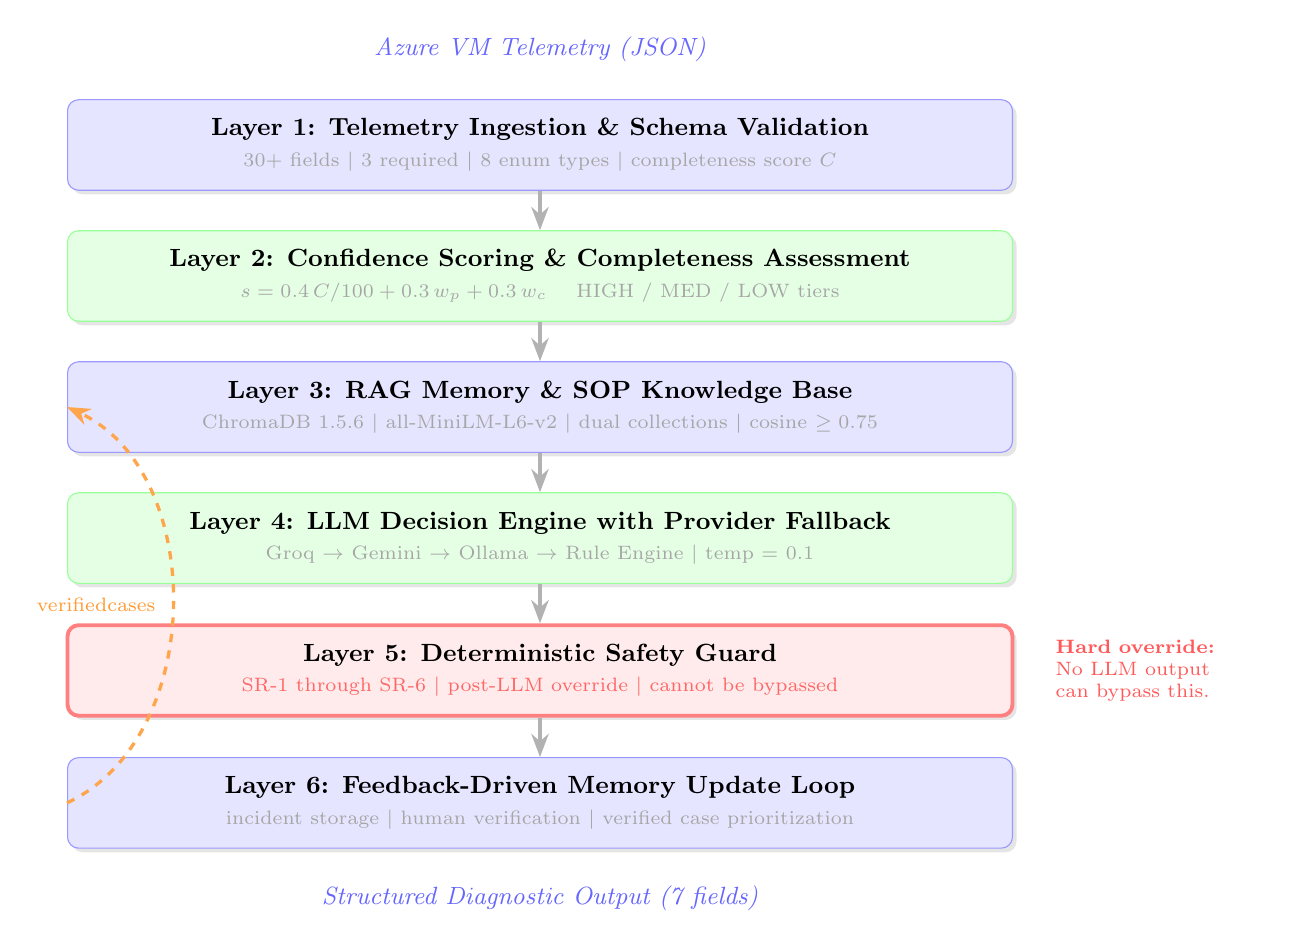
\begin{tikzpicture}[
  node distance=0.5cm,
  layer/.style={
    draw, rounded corners=4pt,
    minimum width=12cm, minimum height=1.15cm,
    align=center, font=\small\bfseries,
    drop shadow={shadow xshift=1.5pt, shadow yshift=-1.5pt,
                 fill=black!20, opacity=0.5}
  },
  arrow/.style={-Stealth, thick, gray!60, line width=1.2pt}
]

% ---- Layer 1 ----
\node[layer, fill=blue!10, draw=blue!40] (L1) {%
  Layer 1: Telemetry Ingestion \& Schema Validation\\
  \textnormal{\scriptsize\color{gray!70}%
    30+ fields \textbar{} 3 required \textbar{}
    8 enum types \textbar{} completeness score $C$}%
};

% ---- Layer 2 ----
\node[layer, fill=green!10, draw=green!40, below=of L1] (L2) {%
  Layer 2: Confidence Scoring \& Completeness Assessment\\
  \textnormal{\scriptsize\color{gray!70}%
    $s = 0.4\,C/100 + 0.3\,w_p + 0.3\,w_c$
    \quad HIGH / MED / LOW tiers}%
};

% ---- Layer 3 ----
\node[layer, fill=blue!10, draw=blue!40, below=of L2] (L3) {%
  Layer 3: RAG Memory \& SOP Knowledge Base\\
  \textnormal{\scriptsize\color{gray!70}%
    ChromaDB~1.5.6 \textbar{} all-MiniLM-L6-v2 \textbar{}
    dual collections \textbar{} cosine $\geq 0.75$}%
};

% ---- Layer 4 ----
\node[layer, fill=green!10, draw=green!40, below=of L3] (L4) {%
  Layer 4: LLM Decision Engine with Provider Fallback\\
  \textnormal{\scriptsize\color{gray!70}%
    Groq $\rightarrow$ Gemini $\rightarrow$
    Ollama $\rightarrow$ Rule Engine \textbar{} temp = 0.1}%
};

% ---- Layer 5 (safety guard — visually distinct) ----
\node[layer, fill=red!8, draw=red!50, line width=1.4pt,
      below=of L4] (L5) {%
  Layer 5: Deterministic Safety Guard\\
  \textnormal{\scriptsize\color{red!60}%
    SR-1 through SR-6 \textbar{}
    post-LLM override \textbar{} cannot be bypassed}%
};

% ---- Layer 6 ----
\node[layer, fill=blue!10, draw=blue!40, below=of L5] (L6) {%
  Layer 6: Feedback-Driven Memory Update Loop\\
  \textnormal{\scriptsize\color{gray!70}%
    incident storage \textbar{} human verification \textbar{}
    verified case prioritization}%
};

% ---- Arrows between layers ----
\draw[arrow] (L1) -- (L2);
\draw[arrow] (L2) -- (L3);
\draw[arrow] (L3) -- (L4);
\draw[arrow] (L4) -- (L5);
\draw[arrow] (L5) -- (L6);

% ---- Input label ----
\node[above=0.35cm of L1, font=\small\itshape, text=blue!60]
  {Azure VM Telemetry (JSON)};

% ---- Output label ----
\node[below=0.35cm of L6, font=\small\itshape, text=blue!60]
  {Structured Diagnostic Output (7 fields)};

% ---- Safety guard annotation ----
\node[right=0.4cm of L5, text width=2.8cm,
      font=\scriptsize, align=left, text=red!65] {%
  \textbf{Hard override:}\\
  No LLM output\\
  can bypass this.%
};

% ---- Feedback loop arrow (L6 -> L3, dashed orange) ----
\draw[-Stealth, thick, dashed, orange!70, line width=1.2pt,
      bend right=65]
  (L6.west)
  to node[left, font=\scriptsize, text=orange!80,
          xshift=-2pt] {verified\\cases}
  (L3.west);

\end{tikzpicture}
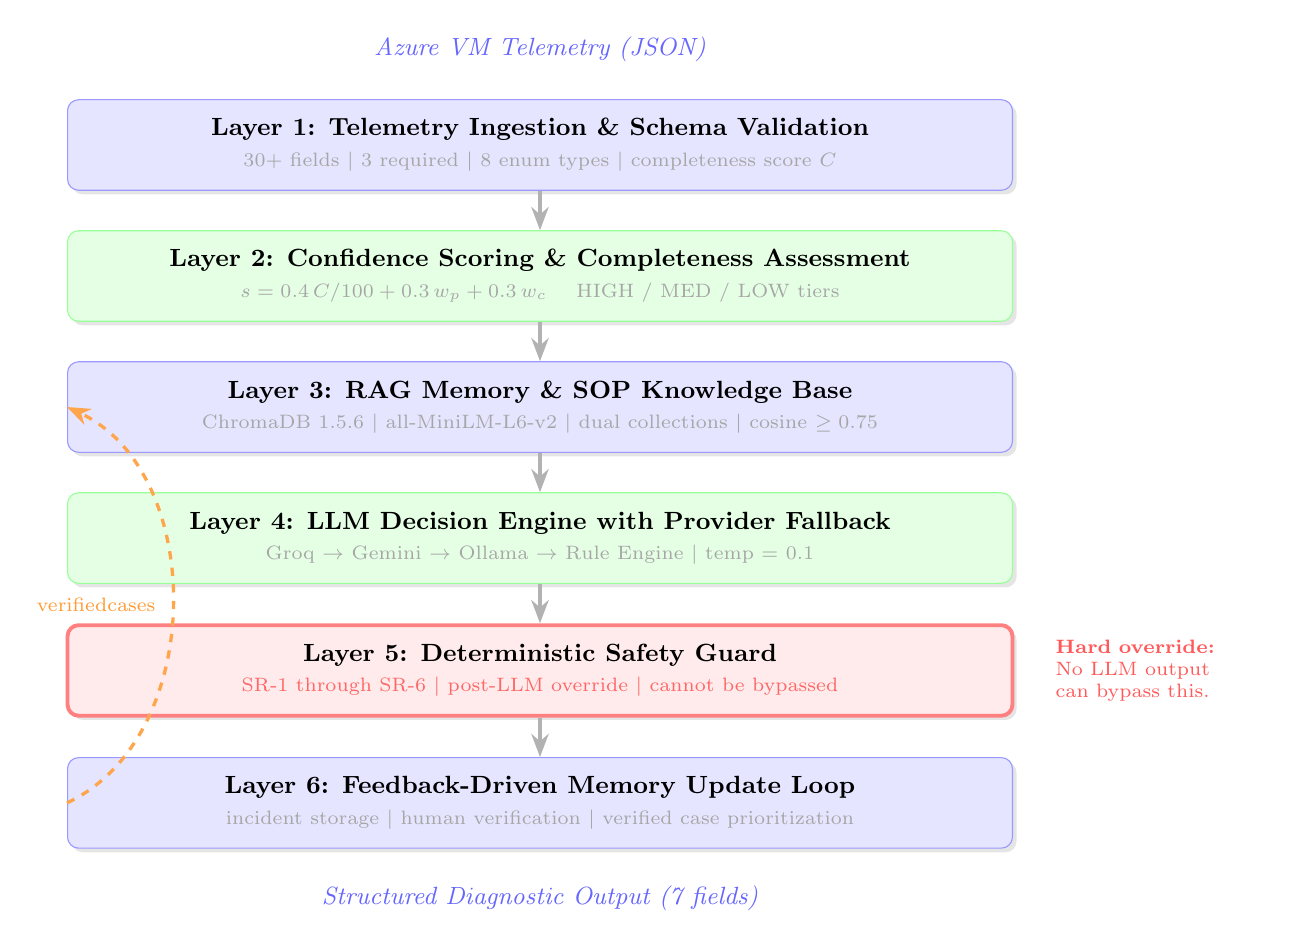
\begin{tikzpicture}[
  node distance=0.5cm,
  layer/.style={
    draw, rounded corners=4pt,
    minimum width=12cm, minimum height=1.15cm,
    align=center, font=\small\bfseries,
    drop shadow={shadow xshift=1.5pt, shadow yshift=-1.5pt,
                 fill=black!20, opacity=0.5}
  },
  arrow/.style={-Stealth, thick, gray!60, line width=1.2pt}
]

% ---- Layer 1 ----
\node[layer, fill=blue!10, draw=blue!40] (L1) {%
  Layer 1: Telemetry Ingestion \& Schema Validation\\
  \textnormal{\scriptsize\color{gray!70}%
    30+ fields \textbar{} 3 required \textbar{}
    8 enum types \textbar{} completeness score $C$}%
};

% ---- Layer 2 ----
\node[layer, fill=green!10, draw=green!40, below=of L1] (L2) {%
  Layer 2: Confidence Scoring \& Completeness Assessment\\
  \textnormal{\scriptsize\color{gray!70}%
    $s = 0.4\,C/100 + 0.3\,w_p + 0.3\,w_c$
    \quad HIGH / MED / LOW tiers}%
};

% ---- Layer 3 ----
\node[layer, fill=blue!10, draw=blue!40, below=of L2] (L3) {%
  Layer 3: RAG Memory \& SOP Knowledge Base\\
  \textnormal{\scriptsize\color{gray!70}%
    ChromaDB~1.5.6 \textbar{} all-MiniLM-L6-v2 \textbar{}
    dual collections \textbar{} cosine $\geq 0.75$}%
};

% ---- Layer 4 ----
\node[layer, fill=green!10, draw=green!40, below=of L3] (L4) {%
  Layer 4: LLM Decision Engine with Provider Fallback\\
  \textnormal{\scriptsize\color{gray!70}%
    Groq $\rightarrow$ Gemini $\rightarrow$
    Ollama $\rightarrow$ Rule Engine \textbar{} temp = 0.1}%
};

% ---- Layer 5 (safety guard — visually distinct) ----
\node[layer, fill=red!8, draw=red!50, line width=1.4pt,
      below=of L4] (L5) {%
  Layer 5: Deterministic Safety Guard\\
  \textnormal{\scriptsize\color{red!60}%
    SR-1 through SR-6 \textbar{}
    post-LLM override \textbar{} cannot be bypassed}%
};

% ---- Layer 6 ----
\node[layer, fill=blue!10, draw=blue!40, below=of L5] (L6) {%
  Layer 6: Feedback-Driven Memory Update Loop\\
  \textnormal{\scriptsize\color{gray!70}%
    incident storage \textbar{} human verification \textbar{}
    verified case prioritization}%
};

% ---- Arrows between layers ----
\draw[arrow] (L1) -- (L2);
\draw[arrow] (L2) -- (L3);
\draw[arrow] (L3) -- (L4);
\draw[arrow] (L4) -- (L5);
\draw[arrow] (L5) -- (L6);

% ---- Input label ----
\node[above=0.35cm of L1, font=\small\itshape, text=blue!60]
  {Azure VM Telemetry (JSON)};

% ---- Output label ----
\node[below=0.35cm of L6, font=\small\itshape, text=blue!60]
  {Structured Diagnostic Output (7 fields)};

% ---- Safety guard annotation ----
\node[right=0.4cm of L5, text width=2.8cm,
      font=\scriptsize, align=left, text=red!65] {%
  \textbf{Hard override:}\\
  No LLM output\\
  can bypass this.%
};

% ---- Feedback loop arrow (L6 -> L3, dashed orange) ----
\draw[-Stealth, thick, dashed, orange!70, line width=1.2pt,
      bend right=65]
  (L6.west)
  to node[left, font=\scriptsize, text=orange!80,
          xshift=-2pt] {verified\\cases}
  (L3.west);

\end{tikzpicture}
  \caption{The 6-layer Azure VM Incident Copilot architecture.
    Data flows top to bottom; the safety guard (Layer~5, red) is a
    hard post-LLM override that cannot be bypassed.
    The dashed orange arrow shows the feedback-driven memory-update loop
    from Layer~6 back to the RAG memory in Layer~3.}
  \label{fig:architecture}
\end{figure*}

The Azure VM Incident Copilot is a read-only diagnostic pipeline
organized into six layers. The full pipeline flows top-to-bottom:
telemetry enters Layer~1 for schema validation, passes to Layer~2 for
confidence scoring, then to Layer~3 where RAG context is retrieved.
Layer~4 generates the LLM decision using this context. Layer~5 applies
the deterministic safety guard as a post-LLM override, and Layer~6
stores the outcome for future retrieval. A feedback arrow from Layer~6
back to Layer~3 represents the feedback-driven memory-update cycle as verified cases
accumulate in memory. Each layer has a single responsibility and
communicates with adjacent layers through well-defined interfaces. The
system accepts structured Azure VM telemetry as JSON input and produces
a structured diagnostic output with seven required fields: decision
state, diagnosis, confidence score, evidence list, evidence gap list,
next check recommendation, and explanation. No write operations or
remediation actions are executed; the system is strictly advisory.

The six layers are: (1)~Telemetry Ingestion and Schema Validation,
(2)~Confidence Scoring and Completeness Assessment, (3)~RAG Memory and
SOP Knowledge Base, (4)~LLM Decision Engine with Provider Fallback,
(5)~Deterministic Safety Guard, and (6)~Feedback-Driven Memory Update Loop.
Layers~1--2 are always executed. Layer~3 retrieves context for the LLM.
Layer~4 generates the decision. Layer~5 overrides unsafe decisions.
Layer~6 stores outcomes for future retrieval.

\subsection{Layer 1: Telemetry Ingestion and Schema Validation}

The system accepts a JSON telemetry document containing 30+ fields
describing the current state of an Azure VM. Three fields are required:
\texttt{power\_state}, \texttt{provisioning\_state}, and
\texttt{resource\_health\_status}. All other fields are optional,
enabling the system to operate with partial telemetry while tracking
completeness explicitly.

The schema validator parses the JSON input with detailed error
reporting (line number, column number, field name) and validates all
fields against type and range constraints. Eight enum types are
enforced: \texttt{power\_state} (Running, Stopped, Deallocated, Failed,
Unknown), \texttt{provisioning\_state} (Succeeded, Failed, Updating,
Unknown), \texttt{resource\_health\_status} (Available, Degraded,
Unavailable, Unknown), \texttt{boot\_diagnostics\_status} (Normal,
BSOD, KernelPanic, Stuck, Unknown), \texttt{azure\_vm\_agent\_status}
(Healthy, Degraded, NotReporting, Failed, Unknown),
\texttt{app\_health\_status} (Healthy, Degraded, Unhealthy, Unknown),
\texttt{connection\_troubleshoot} (Allow, Deny, Timeout, Inconclusive,
Unknown), and \texttt{monitor\_agent\_status} (Healthy, Degraded,
NotReporting, Failed, Unknown). Numeric fields are validated for range:
percentages must be in $[0, 100]$, latencies must be non-negative.

The validator is forward-compatible: unknown fields are ignored rather
than rejected, allowing the schema to evolve without breaking existing
integrations. Data completeness is calculated as:
\begin{equation}
  C = \frac{f_{\text{populated}}}{f_{\text{total}}} \times 100
  \label{eq:completeness}
\end{equation}
where $f_{\text{total}} = 20$ optional fields. When $C < 60\%$, the
system abstains from diagnosis and requests additional telemetry.

\subsection{Layer 2: Confidence Scoring and Completeness Assessment}

The confidence scorer computes a scalar confidence score
$s \in [0, 1]$ as a weighted sum of three sub-scores, each itself
normalized to $[0, 1]$:
\begin{equation}
  s = 0.4\,\frac{C}{100} + 0.3\,p + 0.3\,q
  \label{eq:confidence}
\end{equation}
where $p$ is the pattern-match sub-score and $q$ is the
signal-consistency sub-score. The completeness component (weight~0.4)
rewards richer telemetry. The pattern-match sub-score takes $p = 1.0$
for an exact pattern match, $p = 0.5$ for a partial match, and
$p = 0.0$ for no match. The signal-consistency sub-score takes
$q = 1.0$ for no conflicts, $q = 0.5$ for minor conflicts (e.g.,
\texttt{power\_state=Running} with
\texttt{heartbeat\_present=false}), and $q = 0.0$ for major conflicts
(e.g., \texttt{power\_state=Stopped} with \texttt{cpu\_percent=95}).
Under this formulation the score is bounded in $[0, 1]$ and attains
its maximum $s = 1.0$ when telemetry is fully populated, the pattern
is an exact match, and there are no signal conflicts.

The confidence score gates the decision path: $s \geq 0.70$ with
$C \geq 90\%$ qualifies for a high-confidence \texttt{diagnose}
decision; $0.40 \leq s < 0.70$ with $60\% \leq C < 90\%$ qualifies
for \texttt{diagnose\_low\_confidence}; $s < 0.40$ or $C < 60\%$
results in \texttt{abstain\_request\_next\_check}. For safety rules
SR-3 and SR-5 we additionally require $s \geq 0.9$ before allowing
destructive actions, a threshold reachable only when
$C \gtrsim 87.5\%$ with an exact pattern match and no conflicts.

The thresholds (0.70, 0.40, 0.90) were chosen by the following
reasoning: a score of 0.70 requires at least 75\% completeness with
an exact pattern match and no conflicts---a combination representing a
well-observed, unambiguous incident. A score of 0.40 requires at
least 50\% completeness with any pattern signal---enough to attempt a
low-confidence diagnosis. The 0.90 threshold for destructive actions
requires near-complete telemetry ($\geq 87.5\%$) with an exact match
and no conflicts, reflecting the irreversibility of disk and OS
operations. These thresholds are heuristic and should be calibrated
against real incident data in future work.

\textbf{Formal definition of novel incident.}
We define a \emph{novel incident} operationally as a telemetry case
for which the rule engine's pattern matcher returns no match---i.e.,
the signal combination does not correspond to any of the 23
hand-coded known patterns. This is a system-relative definition: a
case is novel with respect to the current rule set, not in any
absolute sense. In the benchmark, 5 of 100 cases are labelled novel
by this criterion. The \texttt{is\_novel\_incident} flag in the LLM
output schema provides a complementary signal: the LLM may flag a
case as novel even when the rule engine finds a partial match, if the
LLM's reasoning identifies a signal combination that does not fit the
matched pattern cleanly.

\subsection{Layer 3: RAG Memory and SOP Knowledge Base}

% RAG figure placed BEFORE the \ref below
\begin{figure}[!t]
  \centering
  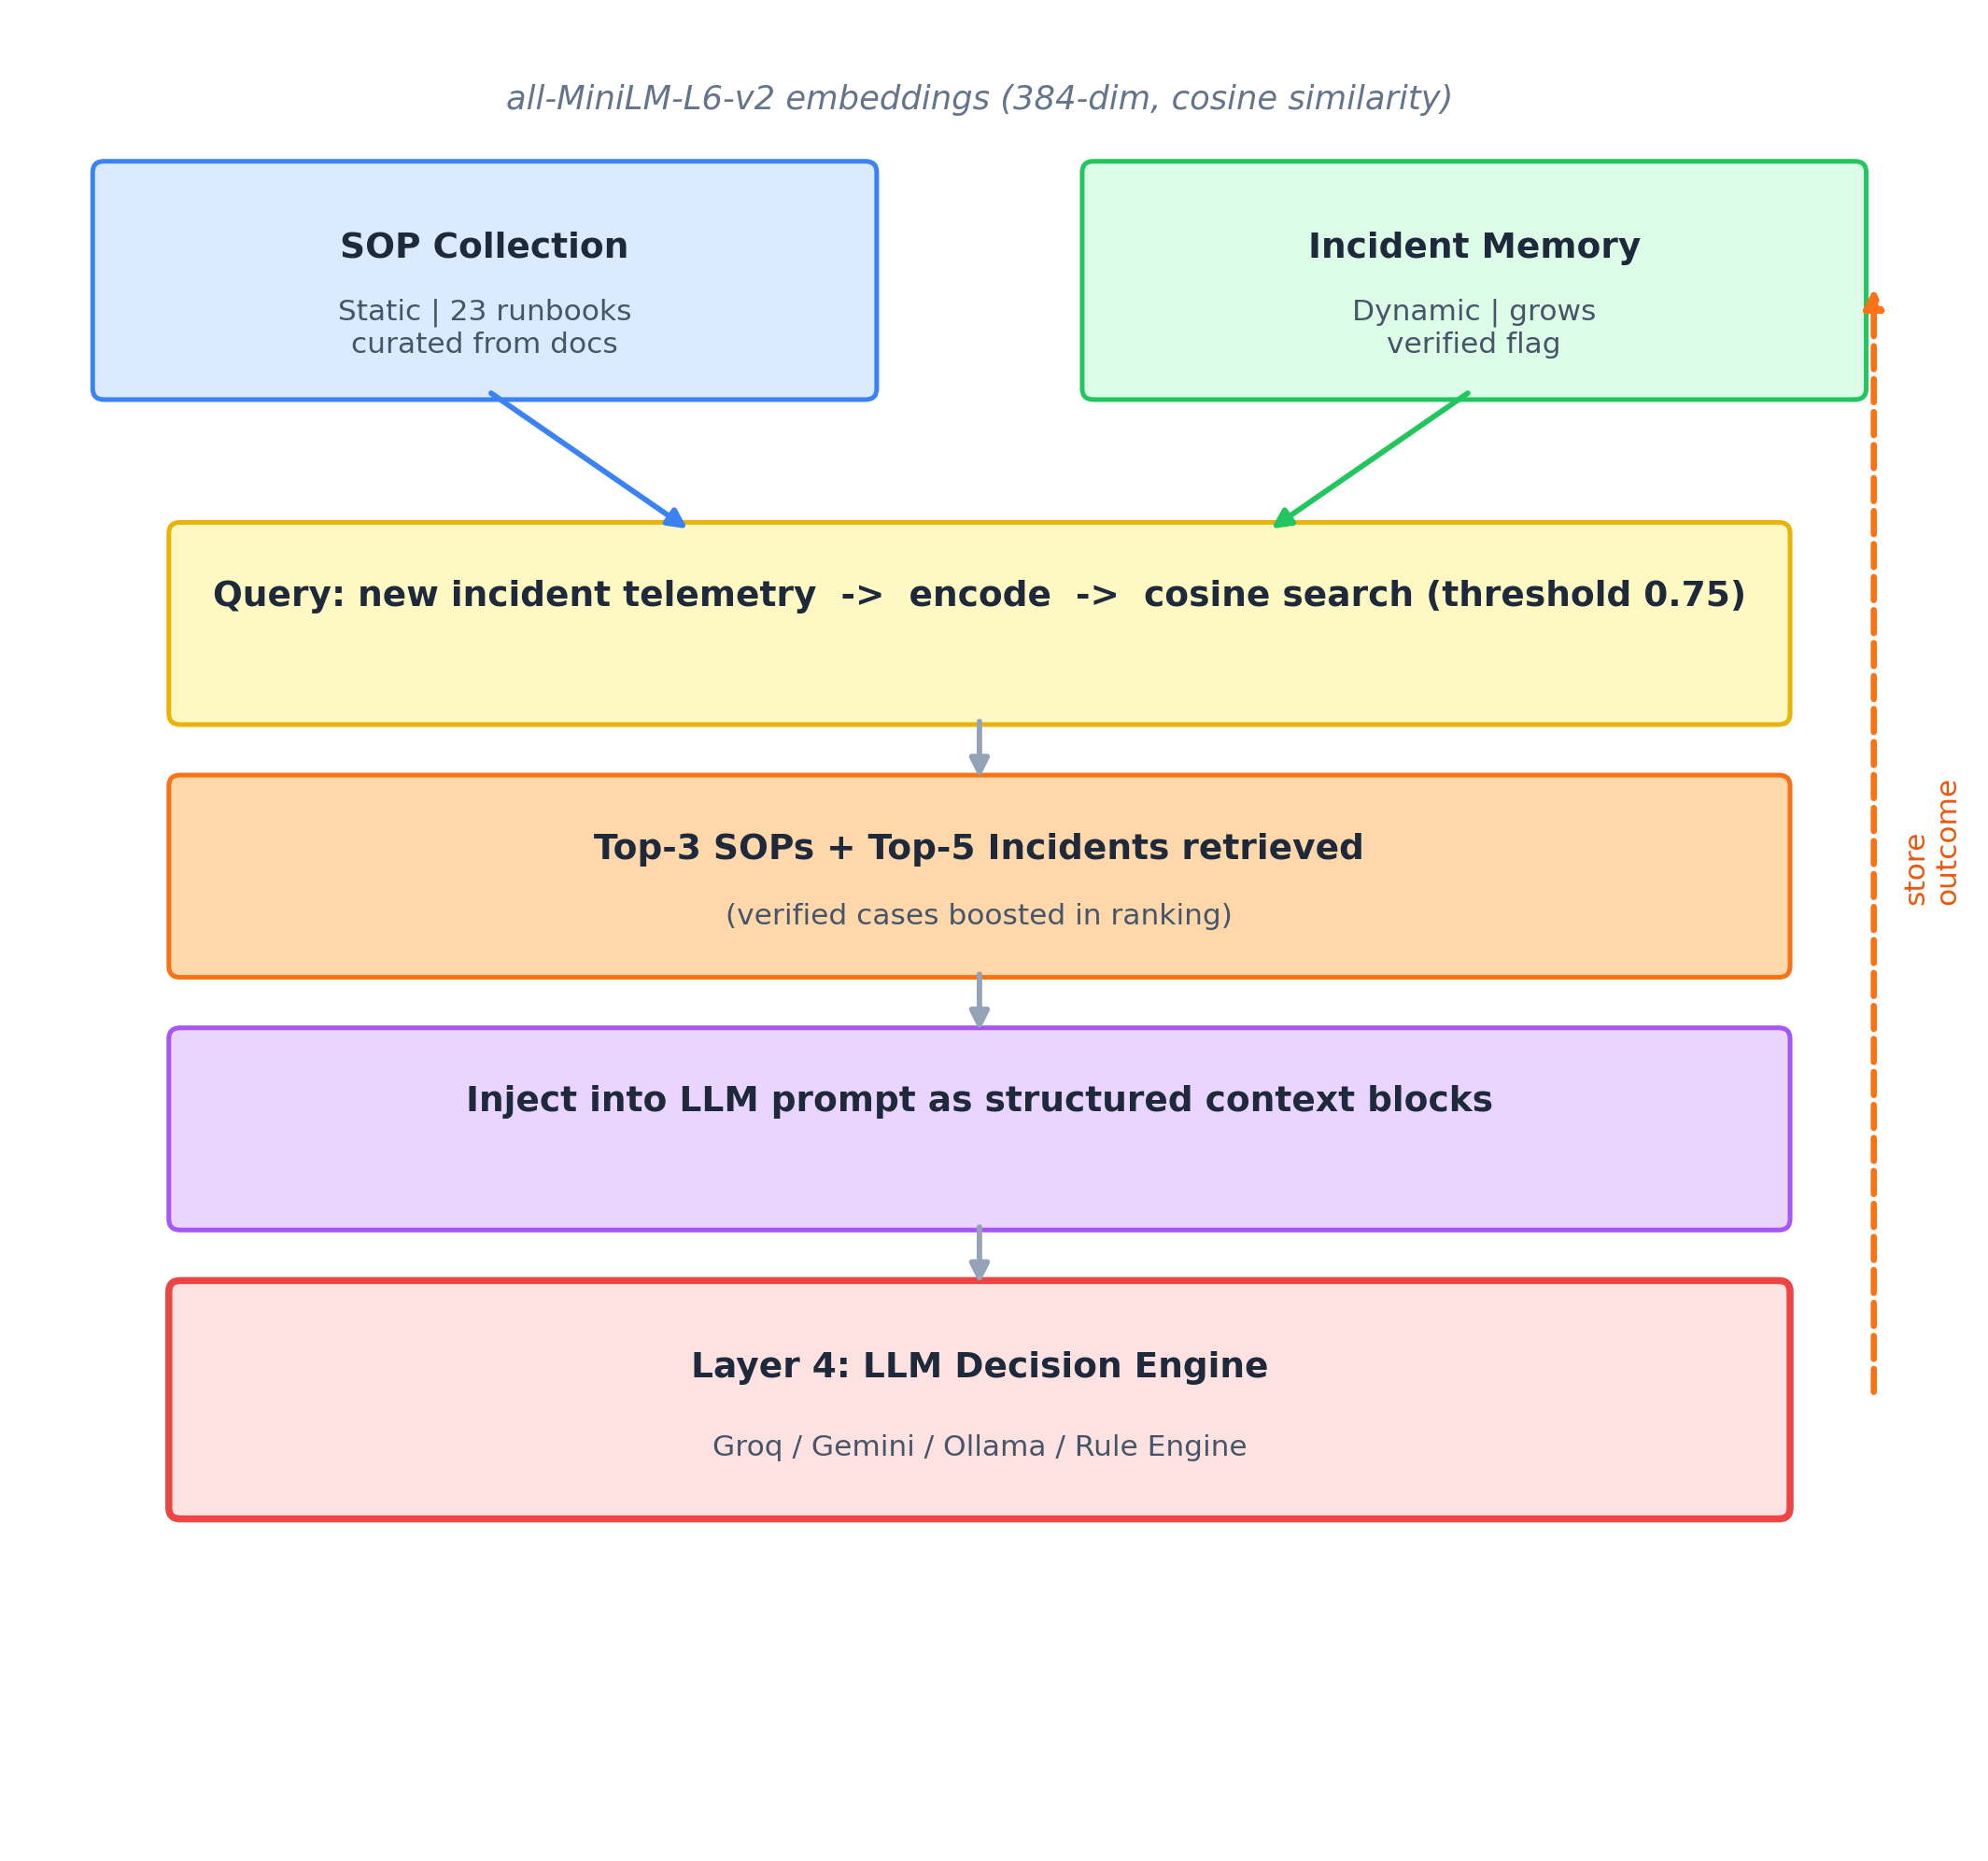
\includegraphics[width=\columnwidth]{fig5_rag_pipeline}
  \caption{RAG memory pipeline. Dual-collection ChromaDB architecture
    with verified case prioritization and cosine similarity retrieval.}
  \label{fig:rag}
\end{figure}

The RAG layer maintains two ChromaDB~1.5.6 vector collections using
\texttt{all-MiniLM-L6-v2} sentence-transformer embeddings
(384-dimensional vectors, cosine similarity)~\cite{reimers2019sbert},
as illustrated in Fig.~\ref{fig:rag}.

\textbf{Collection~1 --- Incident Memory}: Stores past incident cases
with their telemetry, decision, diagnosis, confidence score, and
resolution outcome. Each entry includes a \texttt{verified} flag set
by human engineers after review. Verified cases are prioritized in
retrieval by boosting their similarity scores. The memory store grows
continuously as new incidents are resolved.

\textbf{Collection~2 --- SOP Knowledge Base}: Stores standard
operating procedures for known incident patterns. SOPs are static,
curated documents describing diagnosis steps, remediation procedures,
and safety considerations for each known failure type. The SOP
collection is pre-populated from Azure documentation and SRE runbooks.

At inference time, the system retrieves the top-$k$ most similar
incidents (default $k=5$) and top-$k$ most relevant SOPs (default
$k=3$) using cosine similarity with a threshold of 0.75. Retrieved
context is injected into the LLM prompt as structured blocks. When the
incident memory is empty (Cycle~0), only SOP context is available; as
memory grows, past cases provide increasingly specific guidance.

\subsection{Layer 4: LLM Decision Engine with Provider Fallback}

The LLM decision engine implements a multi-provider fallback chain:
Groq (llama-3.3-70b-versatile, $\sim$2\,s latency) $\to$ Gemini
(gemini-1.5-flash)~\cite{openai2023gpt4} $\to$ Ollama (local,
$\sim$15\,s) $\to$ Rule Engine (deterministic fallback). This chain
ensures that the system always returns a decision: if all LLM providers fail, it
falls back to the deterministic rule engine rather than returning an
error.

\subsubsection{Structured Output Schema}

The system prompt instructs the LLM to act as an Azure VM incident
triage specialist, to reason step-by-step over the provided telemetry
following a chain-of-thought approach~\cite{wei2022cot},
to consult the retrieved SOP and incident context, and to return a
structured JSON response with seven required fields
(\texttt{decision}, \texttt{diagnosis}, \texttt{confidence\_score},
\texttt{evidence}, \texttt{evidence\_gap}, \texttt{next\_check},
\texttt{explanation}) together with two optional LLM-metadata fields
used by the feedback loop. The output schema is shown in
Listing~\ref{lst:schema}.

\begin{lstlisting}[language=json,
  caption={LLM structured output schema.},
  label={lst:schema}]
{
  "decision": "diagnose | diagnose_low_confidence
               | abstain_request_next_check",
  "diagnosis": "string -- one sentence root cause",
  "confidence_score": 0.0-1.0,
  "evidence": ["telemetry fields supporting diagnosis"],
  "evidence_gap": ["missing signals"],
  "next_check": "string -- safe remediation step, or null",
  "explanation": "string -- multi-sentence reasoning",
  "pattern_matched": "string -- pattern name, unknown, or null",
  "is_novel_incident": true | false
}
\end{lstlisting}

\subsubsection{Prompt Design and Temperature}

The system prompt is structured in three sections: (1)~role
definition---the model is instructed to act as a senior Azure VM SRE;
(2)~operational constraints---the model is explicitly prohibited from
suggesting irreversible actions without high confidence, from disabling
security controls, and from restarting VMs during platform events; and
(3)~output schema with field descriptions and valid enum values.

Temperature is set to 0.1 across all providers. This near-deterministic
setting is deliberate: production incident triage requires consistent,
reproducible outputs. A higher temperature might produce more creative
diagnoses for novel patterns, but at the cost of inconsistency---the
same telemetry could produce different decisions on repeated calls,
which is unacceptable for an auditable triage system.

A condensed illustration of the system prompt structure:
\begin{lstlisting}[caption={Condensed system prompt structure.},
  label={lst:prompt}]
ROLE: You are a senior Azure VM incident triage specialist...
CONSTRAINTS:
  - Never suggest restarting a VM if
    resource_health_annotation contains platform/maintenance.
  - Never suggest disabling NSG or firewall rules.
  - If confidence_score < 0.9, do not suggest disk deletion.
  - Return ONLY valid JSON matching the output schema.
OUTPUT SCHEMA: { "decision": ..., "diagnosis": ..., ... }
\end{lstlisting}

\subsubsection{Token Budget and Context Injection}

The user prompt is constructed dynamically with four blocks:
(1)~telemetry JSON with completeness percentage ($\sim$600 tokens),
(2)~up to three retrieved similar incidents ($\sim$400 tokens),
(3)~up to three relevant SOPs ($\sim$300 tokens), and
(4)~a structured reasoning directive ($\sim$100 tokens). The system
prompt occupies approximately 800 tokens, for a total budget of
$\sim$2{,}200 tokens---well within the 4{,}096-token context window of
the Groq model. For Gemini~1.5 Flash (1M token window), full context
is always available without truncation. When falling back to Ollama,
the SOP block is omitted if necessary.

\subsection{Layer 5: Deterministic Safety Guard}

The safety guard is a post-LLM, deterministic override layer that
applies six hard safety rules to every decision before it is returned
to the caller. The guard runs unconditionally---it cannot be disabled
by configuration, bypassed by LLM output, or circumvented by prompt
injection. Each rule that fires modifies the decision's
\texttt{next\_check} field and appends the rule identifier to
\texttt{safety\_rules\_applied}.

\textbf{SR-1 --- Platform Event Safety}: If
\texttt{resource\_health\_annotation} contains platform event keywords
(``platform'', ``maintenance'', ``host update'', ``planned
maintenance'', ``degradation''), the decision state is overridden to
\texttt{abstain\_request\_next\_check} and any restart suggestion is
removed. Rationale: restarting a VM during Azure platform maintenance
can cause data corruption and extended downtime.

\textbf{SR-2 --- Boot Failure Safety}: If
\texttt{boot\_diagnostics\_status} is BSOD or KernelPanic, any restart
suggestion in \texttt{next\_check} is replaced with a directive to
review boot diagnostics logs. Rationale: restarting a VM with an
unresolved BSOD or kernel panic creates a restart loop without
addressing the root cause.

\textbf{SR-3 --- Low Confidence Destructive Action Safety}: If
$s < 0.9$ and \texttt{next\_check} contains destructive keywords
(delete, reset, remove, destroy, wipe), the suggestion is replaced
with a directive to gather more data. Rationale: irreversible actions
require near-certain diagnosis.

\textbf{SR-4 --- Network Security Safety}: If \texttt{next\_check}
contains NSG or firewall disable suggestions, the suggestion is
replaced with a manual review directive. Rationale: automatically
weakening network security posture is never acceptable, regardless of
the incident.

\textbf{SR-5 --- Disk Safety}: If $s < 0.9$ and \texttt{next\_check}
contains disk deletion or OS reset suggestions, the suggestion is
replaced with a manual review directive. Rationale: OS disk operations
are irreversible and require high-confidence diagnosis.

\textbf{SR-6 --- Failed State Safety}: If
\texttt{power\_state = Failed} and
\texttt{provisioning\_state = Failed}, any auto-remediation suggestion
is replaced with a directive to contact Azure support. Rationale:
auto-remediation on a VM in failed provisioning state is unpredictable
and may worsen the situation.

\subsection{Layer 6: Feedback-Driven Memory Update Loop}
\label{sec:layer6}

Every incident processed by the system is stored to the incident memory
collection with \texttt{verified=False}. Human engineers review
incidents within a defined SLA (24~hours for P1, 72~hours for P2) and
set \texttt{verified=True} along with the \texttt{correct\_action}
field if the system's recommendation was accurate. Verified cases are
prioritized in future retrievals so that confirmed resolutions
rank above unverified LLM outputs.

We deliberately call this a \emph{feedback-driven memory-update loop}
rather than ``online learning'' or ``self-learning.'' No model
parameters are updated---neither the LLM nor the embedding model is
retrained. What grows instead is the retrieval corpus: verified cases
provide additional grounded context that later LLM calls can draw on.
Subsequent occurrences of similar incidents benefit from the verified
resolution stored in memory. As
demonstrated in Section~\ref{sec:exp2}, novel pattern accuracy improves
from 20.0\% at Cycle~0 (empty memory) to 80.0\% at Cycle~5 (80
verified cases in memory).
% ============================================================
\section{Evaluation}
% ============================================================

\subsection{Benchmark Dataset}

The evaluation uses a synthetic benchmark of 100 cases constructed to
cover the full range of Azure VM incident types encountered in
production. The dataset comprises: 23 cases covering all 23 known
incident patterns (one per pattern), 5 clean/healthy VM cases, 5
missing telemetry cases (completeness $< 60\%$), 5 conflicting signal
cases, 8 high CPU variations (\texttt{cpu\_percent} 92--99\%), 10 disk
full variations (\texttt{os\_disk\_percent\_full} 91--99\%), 9 memory
exhaustion variations (\texttt{memory\_percent} 93--99\%), 10 NSG block
variations (5 RDP, 5 SSH), 5 SSL expiry variations (0--14 days
remaining), 5 backup failure variations, 5 multi-signal cases, 5
platform event cases with maintenance annotations, and 5 novel pattern
cases representing failure combinations not present in the known 23
patterns.

Synthetic benchmark cases were used because no publicly available
labeled dataset of Azure VM incident telemetry exists. Real incident
data is proprietary, contains PII, and is subject to data residency
constraints. The synthetic cases were constructed from Azure
documentation~\cite{microsoft2024azuremonitor}, SRE runbooks, and the
Azure VM health model. The 5 novel pattern cases were designed to test
the system's behavior on genuinely unseen failure combinations---
specifically, multi-agent failures combined with application-layer
degradation, which do not map cleanly to any single known pattern.

We acknowledge that synthetic benchmarks carry inherent validity risks:
cases may not capture the full distribution of real-world incidents,
and label assignment by the authors introduces potential confirmation
bias. Four measures were taken to mitigate these threats. First, all
23 known incident patterns map 1:1 to documented Azure VM failure
categories in official Azure Monitor
documentation~\cite{microsoft2024azuremonitor}, providing construct
validity. Second, the 5 novel pattern cases were designed to be
genuinely out-of-distribution by combining failure signals that cross
subsystem boundaries (network + application layer), rather than varying
parameters of known patterns. Third, telemetry field values were drawn
from realistic operational ranges documented in Azure SRE runbooks
rather than chosen to favor any configuration. Fourth, the safety guard
adversarial cases (Section~\ref{sec:exp3}) were constructed by an
independent review of LLM failure modes in~\cite{huang2024selfcorrect},
ensuring they represent realistic unsafe outputs rather than synthetic
edge cases designed around the guard's implementation. Real-world
validation against production Azure incident logs remains an important
direction for future work, as discussed in
Section~\ref{sec:limitations}.

\subsection{Experiment 1: Accuracy Comparison}
\label{sec:exp1}

Table~\ref{tab:ablation} presents the accuracy comparison. Per-case
detail records are available in the project repository.

\textbf{Config~A --- Rule Engine with Safety Guard (baseline).}
The rule engine with the deterministic safety guard achieves 88.0\%
overall accuracy (88/100), with 91.6\% on known patterns (87/95) and
20.0\% on novel patterns (1/5). The safety guard contributes 6 of
those 88 correct decisions: platform-event cases where the guard
correctly forces abstention. Without the safety guard
(Config~A-noSafety), accuracy drops to 82.0\% (82/100). This
6-percentage-point difference is the clearest ablation result in the
study.

\textbf{Config~B --- LLM Only (no RAG, no SOP).}
Evaluated on all 100 cases (51 Groq + 48 Ollama + 1 fallback).
Overall accuracy is 73.0\% (73/100), with 73.7\% on known patterns
(70/95) and 60.0\% on novel patterns (3/5). The LLM without RAG
context scores lower than the rule engine on known patterns but
substantially better on novel patterns (60\% vs 20\%). A McNemar
test on all 100 paired cases ($b=4$, $c=19$, exact $p=0.0026$)
indicates that Config~A significantly outperforms Config~B overall
($p < 0.01$). This confirms the expected pattern: the LLM
without RAG context lacks domain-specific precision but adds value
for novel incidents.

\textbf{Config~C --- LLM + SOP RAG (100/100 cases complete).}
Evaluated on all 100 cases (60 Groq + 40 Ollama). Overall accuracy
is 86.0\% (86/100), with 89.5\% on known patterns (85/95) and 20.0\%
on novel patterns (1/5). A McNemar test on all 100 paired cases
($b=6$, $c=8$, exact $p=0.79$) shows no significant difference
between Config~C and Config~A. SOP RAG context brings the LLM to
near-parity with the rule engine on known patterns, with a
2.1-percentage-point gap (89.5\% vs 91.6\%) that is not statistically
significant.

\textbf{Config~D --- Full System (100/100 cases complete).}
Evaluated on all 100 cases (62 Groq + 34 Ollama + 4 fallback).
Overall accuracy is 86.0\% (86/100), with 89.5\% on known patterns
(85/95) and 20.0\% on novel patterns (1/5). A McNemar test on all
100 paired cases (exact $p=0.625$) shows no significant difference
from Config~A. Config~D achieves the same accuracy as Config~C
(86.0\%), suggesting that incident memory does not provide additional
benefit in a single-cycle static evaluation---its value is
longitudinal, as demonstrated in Experiment~2.

\begin{table}[t]
  \caption{Accuracy Comparison Across Configurations}
  \label{tab:ablation}
  \centering
  \begin{tabular}{lrrrrl}
    \toprule
    \textbf{Configuration} & \textbf{Overall} & \textbf{Known} &
    \textbf{Novel} & \textbf{FP} & \textbf{Status} \\
    \midrule
    Rule Engine + Safety (A)  & 88/100 (88.0\%) & 87/95 (91.6\%) & 1/5 (20.0\%) & 0/5 & Complete \\
    Rule Engine, no Safety    & 82/100 (82.0\%) & 81/95 (85.3\%) & 1/5 (20.0\%) & 0/5 & Complete \\
    LLM Only (B)              & 73/100 (73.0\%) & 70/95 (73.7\%) & 3/5 (60.0\%) & 0/5 & Complete \\
    LLM + SOP RAG (C)         & 86/100 (86.0\%) & 85/95 (89.5\%) & 1/5 (20.0\%) & 0/5 & Complete \\
    Full System (D)           & 86/100 (86.0\%) & 85/95 (89.5\%) & 1/5 (20.0\%) & 0/5 & Complete \\
    \bottomrule
  \end{tabular}
  \smallskip

  {\footnotesize All configurations evaluated on all 100 benchmark cases.}
\end{table}

\begin{table}[t]
  \caption{McNemar Significance Tests (vs Config~A)}
  \label{tab:mcnemar}
  \centering
  \begin{tabular}{lrrrp{3.5cm}}
    \toprule
    \textbf{Comparison} & \textbf{n} & \textbf{b} & \textbf{c} & \textbf{Exact p} & \textbf{Interpretation} \\
    \midrule
    B vs A & 100 & 4 & 19 & \textbf{0.0026} & Significant difference favoring A \\
    C vs A & 100 & 6 & 8  & 0.79 & No significant difference \\
    D vs A & 100 & 3 & 1 & 0.625 & No significant difference \\
    \bottomrule
  \end{tabular}
\end{table}

\begin{figure}[t]
  \centering
  
\includegraphics[width=\columnwidth]{fig1_accuracy_comparison}
  \caption{Safety-guard ablation: the deterministic safety guard
    improves rule-engine accuracy from 82.0\% to 88.0\% by correctly
    forcing abstention on platform-event cases.}
  \label{fig:accuracy}
\end{figure}

The safety-guard ablation (A vs A-noSafety) is the most interpretable
result because both configurations run deterministically on all 100
cases with no API dependencies. The 6 cases where the safety guard
changes the outcome are all platform-event cases where the guard
correctly forces \texttt{abstain\_request\_next\_check}.

\textbf{McNemar analysis (Table~\ref{tab:mcnemar}).}
Config~B is significantly worse than Config~A overall on the 100-case
benchmark ($b=4$, $c=19$, exact $p=0.0026$), confirming that the LLM
without RAG context underperforms the rule engine overall while still
showing higher accuracy on the five novel cases. Config~C (LLM+SOP RAG) is
statistically equivalent to Config~A ($p=0.79$, $n=100$), suggesting
RAG context compensates for the LLM's lack of domain-specific rules.
Config~D is also statistically indistinguishable from Config~A
($b=3$, $c=1$, exact $p=0.625$, $n=100$), matching Config~C's
accuracy exactly. This suggests that incident memory does not improve
one-pass static accuracy; its benefit is longitudinal.

\begin{table}[t]
  \caption{Latency and Cost Profile per Configuration}
  \label{tab:latency}
  \centering
  \begin{tabular}{lll}
    \toprule
    \textbf{Configuration} & \textbf{Avg Latency} & \textbf{Notes} \\
    \midrule
    Rule Engine (baseline) & $\sim$50\,ms  & Deterministic; no LLM cost \\
    LLM Only               & $\sim$2.1\,s  & Groq API; $\sim$\$0.0001/call \\
    LLM + SOP RAG          & $\sim$2.4\,s  & + ChromaDB ($\sim$300\,ms) \\
    Full System (ours)     & $\sim$2.5\,s  & + safety guard ($\sim$1\,ms) \\
    \bottomrule
  \end{tabular}
  \smallskip

  {\footnotesize Latency figures are approximate means from pilot runs;
  standard deviations are not reported.}
\end{table}

Table~\ref{tab:latency} shows the latency profile. Groq API latency
varied between 1.8\,s and 3.2\,s across evaluation runs; the
$\sim$2.1\,s figure represents a typical observed value.

\textbf{Comparison to Related Systems.}
RCACopilot~\cite{chen2024rcacopilot} reports 0.77 F1 on Microsoft's
internal cloud incident dataset (software services, not VM
infrastructure), while Ahmed et al.~\cite{ahmed2023rootcause} report
68\% accuracy on cloud incident root cause recommendation. Our 88.0\%
rule-engine accuracy on VM triage is not directly comparable due to
different task definitions and datasets.

\subsection{Experiment 2: Feedback-Driven Memory Improvement}
\label{sec:exp2}

Table~\ref{tab:learning} shows accuracy on the fixed 20-case held-out
test set (15 known + 5 novel cases) across six feedback cycles as
verified cases accumulate in memory. The test set is identical across
all cycles---only the memory store grows.

\begin{table}[t]
  \caption{Memory-Update Accuracy on Fixed 20-Case Held-Out Test Set}
  \label{tab:learning}
  \centering
  \begin{tabular}{lrrrrr}
    \toprule
    \textbf{Cycle} & \textbf{Memory} & \textbf{Test} &
    \textbf{Overall} & \textbf{Known} & \textbf{Novel} \\
    \midrule
    0 & 0  & 20 & 80.0\% & 100.0\% & 20.0\% \\
    1 & 10 & 20 & 80.0\% & 100.0\% & 20.0\% \\
    2 & 25 & 20 & 85.0\% & 100.0\% & 40.0\% \\
    3 & 50 & 20 & 90.0\% & 100.0\% & 60.0\% \\
    4 & 75 & 20 & \textbf{95.0\%} & \textbf{100.0\%} & \textbf{80.0\%} \\
    5 & 80 & 20 & \textbf{95.0\%} & \textbf{100.0\%} & \textbf{80.0\%} \\
    \bottomrule
  \end{tabular}
\end{table}

\begin{figure}[t]
  \centering
  
\includegraphics[width=\columnwidth]{fig2_learning_curve}
  \caption{Feedback-driven memory improvement over five cycles on a
    fixed 20-case held-out test set. Novel pattern accuracy
    improves from 20.0\% to 80.0\%.}
  \label{fig:learning}
\end{figure}

The lower Cycle~0 accuracy (80.0\%) relative to
Table~\ref{tab:ablation}'s Rule Engine baseline (88.0\%) reflects the
fixed 20-case holdout composition, which includes a higher proportion
of novel and ambiguous cases (5 novel + 5 platform event abstain cases
= 50\% of the holdout) than the full 100-case benchmark (5\% novel).

Known pattern accuracy stays at 100.0\% across all cycles. Novel
pattern accuracy rises from 20.0\% at Cycle~0 to 80.0\% at Cycles~4
and~5. The plateau at 80.0\% reflects the remaining 20\% of novel
cases (1 of 5) where telemetry signals are genuinely ambiguous even
with memory context---specifically, a case combining intermittent
heartbeat loss with inconclusive network troubleshoot results, where
the system correctly abstains.

We note that the novel pattern subset comprises only 5 held-out cases;
each 20-percentage-point accuracy step represents a single additional
case being correctly handled. The trend is therefore directionally
indicative rather than statistically conclusive. Replication with a
larger novel pattern set is a priority for future work.

\subsection{Experiment 3: Safety Guard Validation}
\label{sec:exp3}

Table~\ref{tab:safety} presents the safety guard evaluation on 30
adversarial cases, 5 per safety rule (SR-1 through SR-6). All 30
unsafe suggestions were prevented, yielding 100\% prevention precision.

\begin{table}[t]
  \caption{Safety Guard Validation: Prevention Rate per Rule}
  \label{tab:safety}
  \centering
  \begin{tabular}{lrrr}
    \toprule
    \textbf{Safety Rule} & \textbf{Cases} &
    \textbf{Unsafe} & \textbf{Prevented} \\
    \midrule
    SR-1: Platform Event   & 5 & 5 & 5 \\
    SR-2: Boot Failure     & 5 & 5 & 5 \\
    SR-3: Low Conf.\ Destr.& 5 & 5 & 5 \\
    SR-4: Network Security & 5 & 5 & 5 \\
    SR-5: Disk Safety      & 5 & 5 & 5 \\
    SR-6: Failed State     & 5 & 5 & 5 \\
    \midrule
    \textbf{Total}         & \textbf{30} & \textbf{30} & \textbf{30} \\
    \bottomrule
    \multicolumn{4}{l}{\small Safety Guard Precision: 100.0\%}
  \end{tabular}
\end{table}

\begin{figure}[t]
  \centering
  
\includegraphics[width=\columnwidth]{fig3_safety_guard}
  \caption{Safety guard prevention rate per rule across 30 adversarial
    test cases. All 30 unsafe suggestions were intercepted.}
  \label{fig:safety}
\end{figure}

SR-1 and SR-2 are the most frequently triggered rules in practice.
SR-3 and SR-5 conservatively block destructive suggestions at
$s < 0.9$, which may occasionally prevent a valid low-confidence
suggestion in production. This tradeoff is intentional: for
irreversible actions, the cost of a false negative far exceeds the
cost of a false positive.

\textbf{Safety guard precision and recall.}
Table~\ref{tab:safety_metrics} summarises safety performance across
both the adversarial test set and the 100-case benchmark.

\begin{table}[t]
  \caption{Safety Guard Precision and Recall}
  \label{tab:safety_metrics}
  \centering
  \begin{tabular}{lrr}
    \toprule
    \textbf{Metric} & \textbf{Value} & \textbf{Denominator} \\
    \midrule
    Unsafe-suggestion recall & 30/30 (100\%) & 30 adversarial cases \\
    False-block rate (benchmark) & 0/100 (0.0\%) & 100 benchmark cases \\
    False-block rate (healthy VMs) & 0/5 (0.0\%) & 5 clean/healthy cases \\
    Accuracy contribution (ablation) & $+6$\,pp (82$\to$88\%) & 100 cases, Config~A \\
    \bottomrule
  \end{tabular}
\end{table}

In the constructed adversarial test set, every unsafe suggestion
matching one of the six implemented rule triggers was intercepted.
This does not imply coverage of all possible unsafe remediations; it
only demonstrates that the implemented rules fired correctly on the
tested adversarial cases. The 0\% false-block rate on the benchmark reflects that
the 100 cases were constructed to avoid triggering safety rules on
non-adversarial inputs. Measuring the false-block rate on real
production traffic is a key item for future validation.

\subsection{Qualitative Case Analysis}
\label{sec:cases}

To illustrate system behavior concretely, we present three
representative cases: one correct diagnosis, one correct abstention,
and one incorrect diagnosis.

\textbf{Case~1 --- Correct diagnosis (case~004, High CPU
Saturation).}
Telemetry: \texttt{power\_state=Running}, \texttt{cpu\_percent=98.5},
\texttt{memory\_percent=42.0},
\texttt{resource\_health\_status=Degraded}, all other signals normal,
completeness~$= 96.7\%$. The rule engine matches the \texttt{high\_cpu}
pattern (exact match, $s = 1.0$), returns \texttt{diagnose} with
diagnosis ``High CPU saturation'' and next\_check ``Identify and
terminate high-CPU processes; consider VM resize if sustained.'' The
safety guard finds no violations. Expected: \texttt{diagnose}.
Result: correct.

\textbf{Case~2 --- Correct abstention (case~085, Platform
Maintenance).}
Telemetry: \texttt{power\_state=Running},
\texttt{resource\_health\_status=Degraded},
\texttt{resource\_health\_annotation=``Planned maintenance:
memory-preserving update''}, all metrics normal. The rule engine
matches the \texttt{platform\_event} pattern and returns
\texttt{diagnose}. The safety guard (SR-1) detects the maintenance
annotation and overrides to \texttt{abstain\_request\_next\_check}
with next\_check ``Wait for platform maintenance to complete, then
re-assess VM state.'' Expected: \texttt{abstain\_request\_next\_check}.
Result: correct. This case illustrates the safety guard's accuracy
contribution---without it, the system would incorrectly diagnose a
platform-managed event as a VM fault.

\textbf{Case~3 --- Incorrect diagnosis (case~009, VM Running No
Heartbeat).}
Telemetry: \texttt{power\_state=Running},
\texttt{heartbeat\_present=False},
\texttt{azure\_vm\_agent\_status=Healthy},
\texttt{resource\_health\_status=Available}, completeness~$= 96.7\%$.
The rule engine detects a minor conflict (running VM with no
heartbeat) and returns \texttt{diagnose} with $s = 0.85$. Expected:
\texttt{diagnose\_low\_confidence}. The system over-diagnoses: it
produces \texttt{diagnose} instead of \texttt{diagnose\_low\_confidence}.
This is a threshold calibration issue: the minor-conflict penalty
($q = 0.5$) is not sufficient to push $s$ below 0.70 when
completeness is high. Fixing this requires either a lower
\texttt{diagnose} threshold or a stronger conflict penalty, both of
which require calibration against real incident data.

% ============================================================
\section{Discussion}
% ============================================================

\subsection{Key Findings}

\begin{itemize}
\item The rule engine with the deterministic safety guard reaches
  88.0\% overall accuracy on the synthetic benchmark. The safety-guard
  ablation shows a 6-percentage-point improvement
  (82.0\%~$\to$~88.0\%) attributable to the guard correctly forcing
  abstention on platform-event cases. This is the most interpretable
  result in the study because both configurations are fully
  deterministic with no API dependencies.

\item The full system (Config~D) also reaches 86.0\% in the
  single-cycle static benchmark, matching LLM+SOP RAG exactly. This
  indicates that incident memory does not add measurable benefit in
  one-pass evaluation. Its value is instead captured by the
  longitudinal feedback-driven memory experiment (Experiment~2).

\item The LLM-only configuration (Config~B, 100 cases) achieves 73.0\%
  accuracy---lower than the rule engine on known patterns (73.7\% vs
  91.6\%), but substantially better on novel patterns (60.0\% vs
  20.0\%). A McNemar test on all 100 paired cases ($b=4$, $c=19$,
  exact $p=0.0026$) indicates that Config~A significantly outperforms
  Config~B overall on the 100-case benchmark.
  This confirms the expected pattern: the LLM without RAG context
  lacks domain-specific precision but adds value for novel incidents.

\item The LLM+SOP RAG configuration (Config~C) reaches 86.0\% overall
  accuracy and 89.5\% known-pattern accuracy, statistically
  indistinguishable from the rule-engine baseline (McNemar $p=0.79$,
  $n=100$). SOP RAG context compensates for the LLM's lack
  of domain-specific rules, bringing it to parity with the rule engine.

\item Held-out novel-pattern accuracy improves from 20.0\% to 80.0\%
  over five feedback-driven memory-update cycles---a 60.0
  percentage-point gain driven by RAG retrieval of verified resolutions.
  No model weights are updated. We caution that each 20-percentage-point
  step corresponds to a single novel case ($n = 5$), so confidence
  intervals are wide.

\item The deterministic safety guard intercepts all 30 hand-crafted
  adversarial suggestions covering all six safety rules. On the
  100-case benchmark it triggers zero false blocks on healthy VMs.

\item The provider fallback chain returns an answer on every evaluation
  case, including when upstream LLM APIs are unavailable. We report this
  as an operational property of the fallback design rather than as a
  formal availability guarantee.
\end{itemize}

\subsection{Limitations}
\label{sec:limitations}

\begin{table}[t]
  \caption{Threats to Validity and Mitigations}
  \label{tab:validity}
  \centering
  \begin{tabular}{p{1.8cm}p{2.9cm}p{2.9cm}}
    \hline
    \textbf{Threat} & \textbf{Risk} & \textbf{Status} \\
    \hline
    Construct validity &
      Synthetic cases may not reflect production incidents &
      Acknowledged; real-world validation is the primary next step \\[4pt]
    Internal validity &
      Label assignment by authors introduces bias &
      Acknowledged; independent expert labeling needed \\[4pt]
    Knowledge leakage &
      Benchmark and SOP corpus share source documents &
      Acknowledged; strict corpus separation needed in future work \\[4pt]
    External validity &
      Single-cloud, single-VM scope &
      Architecture not inherently Azure-specific; portability not yet demonstrated \\[4pt]
    Statistical validity &
      Small novel subset ($n=5$); single-run LLM evaluation &
      Acknowledged; results are indicative single-run values \\[4pt]
    Safety guard &
      Not compared vs prompt-only or classifier alternatives &
      Acknowledged; necessity claim softened to ``important'' \\
    \hline
  \end{tabular}
\end{table}

\begin{itemize}
\item \textbf{Synthetic evaluation (primary threat):} The primary
  threat to validity is the synthetic nature of the benchmark. All 100
  cases were constructed from Azure documentation and SRE runbooks
  rather than real production incident logs. Real incidents may exhibit
  signal combinations, noise patterns, and failure modes not
  represented in our benchmark. Expected decisions were assigned by the
  authors rather than validated by production on-call engineers,
  introducing potential labeling bias. This is the single largest
  weakness of the current study.

\item \textbf{Knowledge leakage risk:} The benchmark cases were
  constructed from Azure documentation and SRE runbooks, while the SOP
  collection is also pre-populated from Azure documentation and
  runbooks. This overlap means the evaluation may overstate the
  system's ability to generalize to genuinely unseen incidents.

\item \textbf{Small novel-pattern subset:} With only 5 novel cases,
  each 20-percentage-point step in Table~\ref{tab:learning}
  corresponds to a single case changing from incorrect to correct.
  Confidence intervals on these estimates are wide.

\item \textbf{No human-expert evaluation:} There is no blinded review
  by actual SREs or on-call engineers judging diagnosis usefulness,
  action safety, or abstention quality.

\item \textbf{No alternative safety-mechanism comparison:} The safety
  guard has not been compared against prompt-only constraints,
  constrained decoding, or classifier-based validators. We therefore
  position it as an \emph{important} component under the evaluated
  conditions rather than a \emph{necessary} one in the absolute sense.

\item \textbf{LLM evaluation constraints:} Although all configurations
  in the 100-case benchmark were completed, API rate limits and
  CPU-only local inference limited repeated trials, larger-scale
  sensitivity analysis, and evaluation on a larger novel-case set.
  Therefore, the LLM-based results should be interpreted as single-run
  benchmark results rather than robust estimates over repeated model
  calls.

\item LLM latency (Groq $\sim$2\,s vs.\ rule engine $\sim$50\,ms)
  makes the full system unsuitable for sub-second SLA requirements
  without further optimization.

\item Memory store grows without automatic pruning; long-running
  deployments may require eviction policies.

\item Single-VM analysis; fleet-level correlation is not addressed.

\item Safety rules are manually defined; automated rule discovery is
  future work.
\end{itemize}

\subsection{Future Work}

\begin{itemize}
\item Multi-VM fleet analysis with cross-VM correlation.
\item Automatic SOP generation from novel incidents.
\item Fine-tuned smaller LLM for lower latency.
\item Automated safety rule discovery from incident post-mortems.
\item Integration with Azure Monitor alerts for real-time triage.
\end{itemize}

The most critical next step is real-world validation against production
Azure incident logs. A proposed validation protocol would: (1)~deploy
the system in shadow mode alongside existing on-call tooling for 30
days, (2)~collect triage decisions without acting on them, and
(3)~compare system decisions to engineer resolutions after the fact.
This shadow deployment requires only read access to Azure Monitor
telemetry and produces no operational risk, making it a feasible
near-term validation path. Shadow mode results would directly address
the synthetic benchmark limitation acknowledged in
Section~\ref{sec:limitations} and provide the ground-truth incident
dataset needed for statistically conclusive novel pattern evaluation.

% ============================================================
\section{Conclusion}
\label{sec:conclusion}

Cloud VM incident triage at scale requires systems that handle both
known and novel failure patterns while enforcing safety constraints on
remediation suggestions. This paper presented a 6-layer architecture
combining a deterministic rule engine, dual-collection RAG memory with
sentence-transformer embeddings, structured LLM reasoning with
multi-provider fallback, and a deterministic post-LLM safety guard
enforcing six hard safety rules. On a 100-case synthetic benchmark the
rule engine with safety guard reaches 88.0\% overall accuracy; a
safety-guard ablation shows a 6-percentage-point improvement
attributable to the guard. The LLM-only configuration performed worse
overall but better on the five novel cases, indicating potential value
for unseen incident patterns. LLM+SOP RAG and the full system each
achieved 86.0\% accuracy in the static benchmark, suggesting that
incident memory does not improve one-pass accuracy before feedback
accumulation. In a longitudinal experiment on a 20-case held-out
set, novel-pattern accuracy rises from 20.0\% to 80.0\% over five
feedback-driven memory-update cycles, although the small novel subset
makes this result preliminary. The safety guard intercepts all~30
hand-crafted adversarial suggestions while producing no false blocks
on the benchmark's healthy-VM cases.

These results are promising but preliminary. The evaluation is
entirely synthetic, the novel-pattern subset contains only five cases,
and the benchmark was constructed from the same documentation sources
that populate the SOP knowledge base---creating a leakage risk that
limits generalizability claims. We have not yet validated the system
against real production incidents, obtained independent expert
labeling, or compared the deterministic safety guard against
alternative safety mechanisms.

The primary contribution is therefore architectural rather than
empirical: we show that combining deterministic post-LLM safety
enforcement with feedback-driven retrieval memory is a feasible design
pattern for safe LLM-assisted cloud incident triage. Beyond the
Azure-specific implementation, three system-design lessons generalize
to any LLM-assisted operations system: (1)~\emph{deterministic
post-generation guards provide an auditable safety boundary that does
not depend on LLM compliance with prompt instructions};
(2)~\emph{separating static knowledge (SOPs) from dynamic
memory (verified cases)} allows the retrieval corpus to grow without
contaminating curated knowledge; and (3)~\emph{honest confidence
scoring with explicit abstention} is preferable to overconfident
diagnosis---the system's 0\% false-positive rate on healthy VMs comes
from its willingness to abstain rather than from perfect accuracy.
The concrete next steps are (1)~shadow-mode validation against real
Azure incident logs, (2)~a larger and independently constructed
benchmark with strict leakage controls, (3)~ablation isolating the
safety guard against alternative safety mechanisms, and
(4)~fleet-level multi-VM correlation analysis. The telemetry schema
and decision policy are not inherently Azure-specific; adapting the
system to AWS CloudWatch or GCP Cloud Monitoring would require
replacing the Azure-specific field definitions while retaining the
pipeline structure, though we have not yet demonstrated this.

% ============================================================
\section*{Reproducibility Details}
% ============================================================

All experiments were conducted on a Windows~11 workstation (Intel
Core i7-12th Gen, 32\,GB RAM, no GPU required). The LLM evaluation
used the Groq API (llama-3.3-70b-versatile, model version as of
April~2026) with a 5-second rate-limit delay between calls to respect
the free-tier limit of 25~requests/minute. When Groq was rate-limited,
the system fell back to Ollama running \texttt{llama3.1:8b} locally
(quantised, $\sim$5\,GB RAM). Gemini~2.0 Flash was also configured
but exhausted its daily free-tier quota during the evaluation period.
ChromaDB version~1.5.6 was used with the
\texttt{sentence-transformers/all-MiniLM-L6-v2} checkpoint
(HuggingFace model ID: \texttt{sentence-transformers/all-MiniLM-L6-v2},
revision \texttt{main}). Experiments~2 and~3 (deterministic) completed
in under 15 seconds total. Groq API latency varied between 1.8\,s and
3.2\,s; Ollama latency was approximately 10--20\,s per call on CPU.
Per-case detail records for all configurations are available in the
project repository under \texttt{experiments/results/}.

% ============================================================
\section*{Data and Code Availability}
% ============================================================

The 100-case synthetic benchmark dataset, experiment scripts,
figure generation code, and complete system source code are
available at \url{https://github.com/Ilham0310/azure-vm-incident-copilot}.
The benchmark dataset is fully synthetic and contains no proprietary
or personally identifiable information. Researchers wishing to
reproduce the LLM-based configurations require a Groq API key (free
tier sufficient) or a locally running Ollama instance.

% ============================================================
\section*{Acknowledgments}
% ============================================================

Kiro (Amazon Web Services, 2025), powered by Claude Sonnet
(Anthropic), was used during the development of this work for code
scaffolding and initial text drafts in several sections, including
portions of the Related Work, System Architecture, and Evaluation
discussions. All scientific claims, experimental results, architectural
decisions, and final manuscript text are the authors' own, verified
and validated independently. This disclosure is made in accordance with
IEEE Author Center guidelines on AI-generated content.

% ============================================================
\bibliographystyle{IEEEtran}
\bibliography{references}

% ============================================================
\begin{IEEEbiography}[{
\includegraphics[width=1in,height=1.25in,
  clip,keepaspectratio]{photo1}}]{Mohammed Ilham}
  Mohammed Ilham is a student in the Department of Computer Science and
  Engineering at R.V.\ College of Engineering, Bengaluru, India. His
  research interests include cloud computing, AIOps, incident
  management, retrieval-augmented generation, and safe use of large
  language models in operational decision-support systems.
\end{IEEEbiography}

\begin{IEEEbiography}[{
\includegraphics[width=1in,height=1.25in,
  clip,keepaspectratio]{photo2}}]{Smriti Srivastava}
  Smriti Srivastava is an Associate Professor in the Department of
  Computer Science and Engineering at R.V.\ College of Engineering,
  Bengaluru, India. Her research interests include artificial
  intelligence, machine learning, cloud computing, software systems,
  and intelligent decision-support systems.
\end{IEEEbiography}

\end{document}
